\documentclass{article}
\usepackage{graphicx}
\usepackage{multirow} 

\begin{document}
\begin{table}[h!]
  \begin{center}
  	\caption{multirow table}
  	\label{tab:table1}
  	\begin{tabular}{l|c|r}
  		\hline
  	  \textbf{value 1} & \textbf{Value 2} & \textbf{value 3}\\
  	  $\alpha$ & $\beta$ & $\gamma$ \\
  	  \hline
  	  \multirow{2}{*}{12} & 1110.l0 & a\\
  	  & 10.10 & b\\
  	  \hline
  	  14 & 25.11 & \multirow{2}{*}{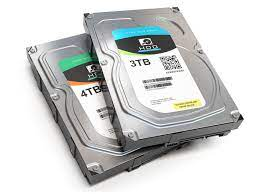
\includegraphics[width=0.07\linewidth]{picture3}}\\
  	  25 & 345.11 & \\
  	  \hline
  	  36 & 35.12 & c \\
  	  \hline
  	  \end{tabular}
   \end{center}
\end{table}

\end{document}